\subsection{Priors on Change-Point Locations}

\label{app:prior}

In the absence of any prior knowledge about the location of the change-point $\tau \in [T]$, one natural choice is the uniform prior, $\pi_t = T^{-1}$. While this choice of $\boldsymbol{\pi}_{1:T}$ satisfies Assumption \ref{assumption:1} (iii) and therefore guarantees asymptotic consistency for each of the single change-point models in Section \ref{sec:scp}, the uniform prior may reduce detection power or even lead to false positives for small $T$. To see this we first show that the uniform prior does not induce a uniform posterior in the absence of a change-point. In Figure \ref{fig:post-probs-plot}, we plot MCMC estimates of $\E[\overline{\pi}_{1:T} \:|\: \mathbf{y}_{1:T}]$ for the three SCP models for a length $T=50$ univariate sequence under the null model, i.e. where $y_t \overset{\text{i.i.d.}}{\sim}\mathcal{N}(0,1)$. 
\begin{figure}[!h]
    \centering
    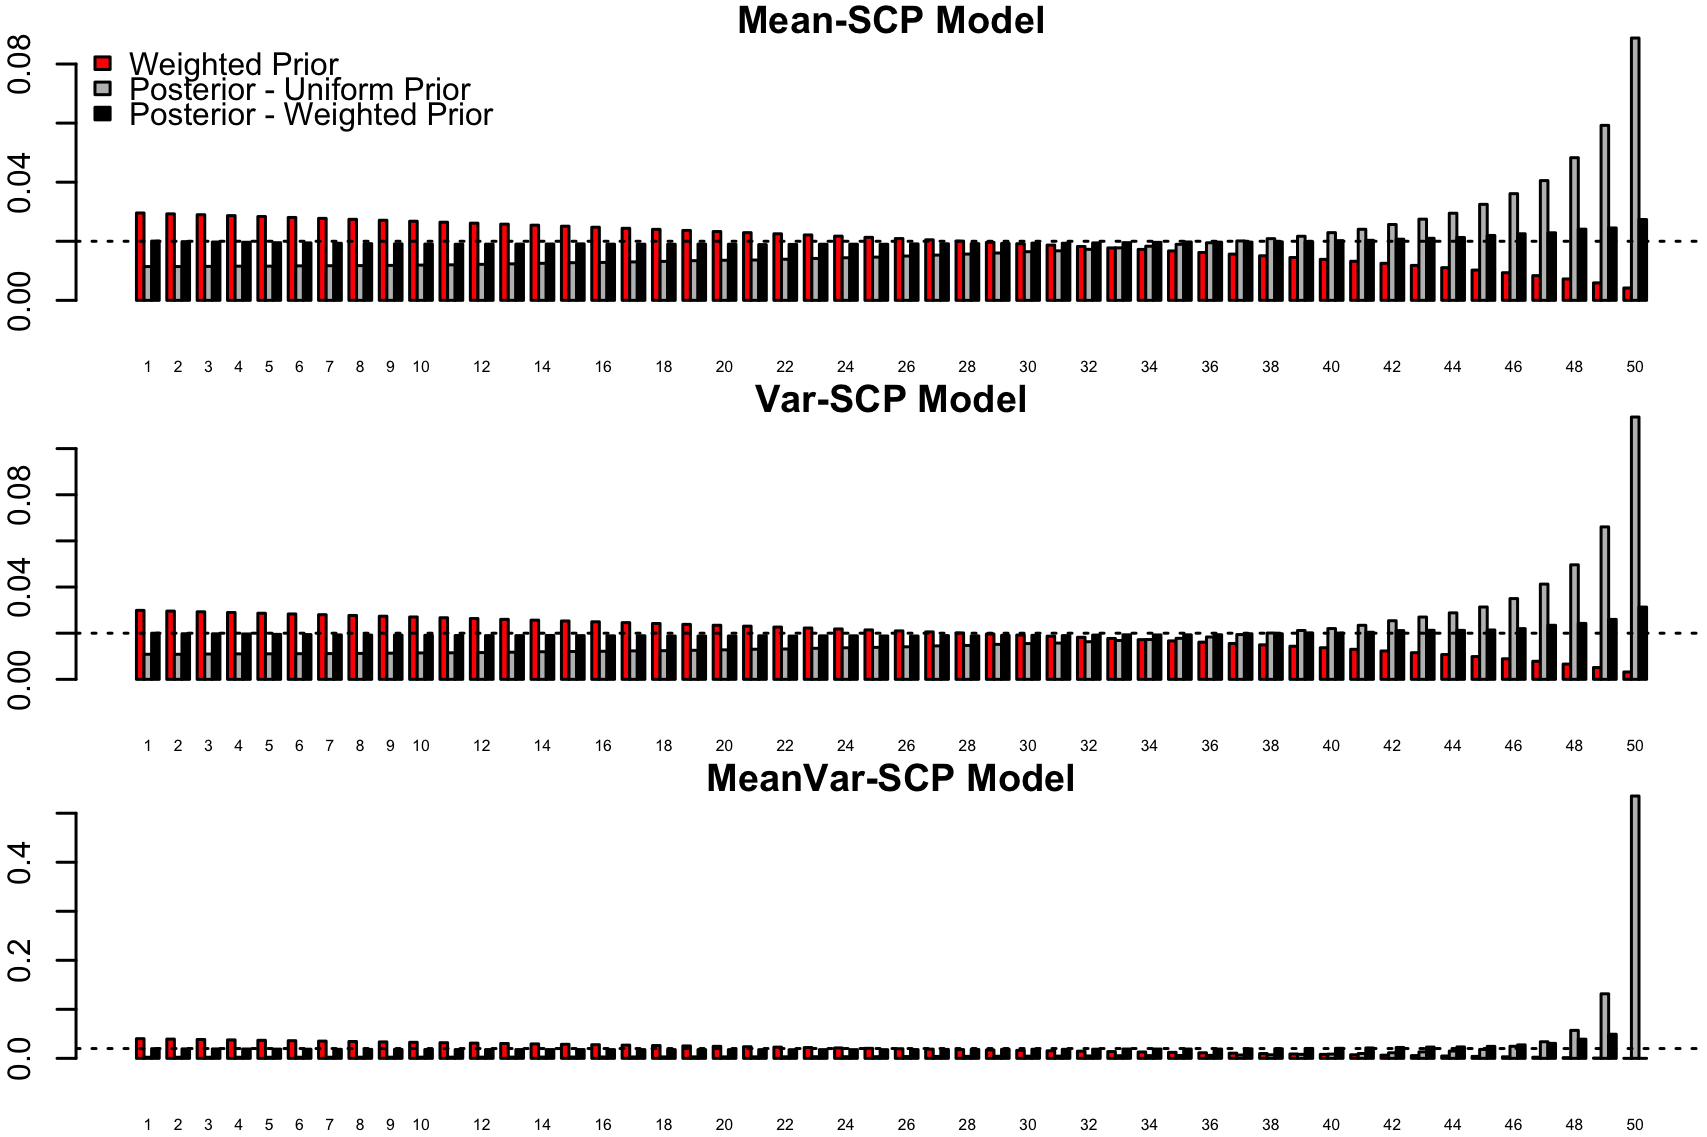
\includegraphics[scale = 0.27]{MICH/Figures/prior_choice_plot.png}
    \caption{$\E[\boldsymbol{\pi}_{1:T}\:|\: \mathbf{y}_{1:T}]$ under Null Model}
    \label{fig:post-probs-plot}
\end{figure}

Figure \ref{fig:post-probs-plot} shows an exponential increase in the posterior probabilities as $t$ approaches $T$. With a uniform prior, the SCP models may fail to detect a true change when the signal is weak or in small samples due to the large weight placed on times near $T$. For the var-scp and meanvar-scp models in particular, we see that the probabilities may be large enough to incorrectly detect a change-point in the vicinity of time $T$, even when no change is present. To rectify this behavior we propose selecting $\boldsymbol{\pi}_{1:T}$ so that under the null model we have:
\begin{align}\label{eq:prior-cond}
    \E\left[\log\overline{\pi}_t - \log \overline{\pi}_{t+1} \right] = 0.
\end{align}
In Figure \ref{fig:post-probs-plot} we also plot the weighted priors $\boldsymbol{\pi}_{1:T}$ that satisfy (\ref{eq:prior-cond}) and MCMC estimates of $\E[\overline{\pi}_{t} \:|\: \mathbf{y}_{1:T}]$ under this choice $\boldsymbol{\pi}_{1:T}$. We clearly see that these estimates adhere much more closely to the uniform dashed line at $T^{-1}$. Note that (\ref{eq:prior-cond}) also implies a uniform condition on the posterior probabilities since for any $r > t$:
\begin{align*}
    \E\left[\log\overline{\pi}_t - \log \overline{\pi}_r \right] &= \sum_{i=0}^{r-t-1} \E\left[\log\overline{\pi}_{t+i} - \log \overline{\pi}_{t+i+1} \right] = 0.
\end{align*}
We now show how to calculate $\pi_t$ so that (\ref{eq:prior-cond}) holds for each of the SCP models. In each case we show that, if $t_0$ is the true location of the change point

\subsubsection{Mean-SCP Prior}

For the mean-scp model in Section \ref{sec:smcp} we have:
\small
\begin{align*}
    \E\left[\log\overline{\pi}_t - \log \overline{\pi}_{t+1} \right] &= \log \pi_t - \log \pi_{t+1} - \frac{1}{2} \log \left|\omega_0\mathbf{I}_d + \sum_{t'=t}^{T} \boldsymbol{\Lambda}_{t'}\right| + \frac{1}{2} \log \left|\omega_0\mathbf{I}_d + \sum_{t'=t+1}^{T} \boldsymbol{\Lambda}_{t'}\right|\\
    &\quad + \frac{1}{2} \E\left[\left\lVert \left[\omega_0\mathbf{I}_d + \sum_{t'=t}^{T} \boldsymbol{\Lambda}_{t'}\right]^{-\frac{1}{2}} \sum_{t'=t}^{T} \boldsymbol{\Lambda}_{t'} \mathbf{y}_{t'}\right\rVert_2^2 \right] - \frac{1}{2} \E\left[\left\lVert \left[\omega_0\mathbf{I}_d + \sum_{t'=t+1}^{T} \boldsymbol{\Lambda}_{t'}\right]^{-\frac{1}{2}} \sum_{t'=t+1}^{T} \boldsymbol{\Lambda}_{t'} \mathbf{y}_{t'}\right\rVert_2^2 \right].
\end{align*}
\normalsize
Letting $\omega_0 \to 0$ and noting that $\sum_{t'=t}^{T} \boldsymbol{\Lambda}_{t'} \mathbf{y}_{t'} \sim \mathcal{N}_d\left(\mathbf{0}, \sum_{t'=t}^{T} \boldsymbol{\Lambda}_{t'}\right)$ under the null model, we get:
\small
\begin{align*}
    \E\left[\log\overline{\pi}_t - \log \overline{\pi}_{t+1} \right] &= \log \pi_t - \log \pi_{t+1} - \frac{1}{2} \log \left|\sum_{t'=t}^{T} \boldsymbol{\Lambda}_{t'}\right| + \frac{1}{2} \log \left|\sum_{t'=t+1}^{T} \boldsymbol{\Lambda}_{t'}\right|\\
    &\quad + \frac{1}{2} \E\left[\left\lVert \left[ \sum_{t'=t}^{T} \boldsymbol{\Lambda}_{t'}\right]^{-\frac{1}{2}} \sum_{t'=t}^{T} \boldsymbol{\Lambda}_{t'} \mathbf{y}_{t'}\right\rVert_2^2  \right] - \frac{1}{2} \E\left[\left\lVert \left[\sum_{t'=t+1}^{T} \boldsymbol{\Lambda}_{t'}\right]^{-\frac{1}{2}} \sum_{t'=t+1}^{T} \boldsymbol{\Lambda}_{t'} \mathbf{y}_{t'}\right\rVert_2^2  \right]\\
    &= \log \pi_t - \log \pi_{t+1} - \frac{1}{2} \log \left|\sum_{t'=t}^{T} \boldsymbol{\Lambda}_{t'}\right| + \frac{1}{2} \log \left|\sum_{t'=t+1}^{T} \boldsymbol{\Lambda}_{t'}\right|.
\end{align*}
\normalsize
If $\boldsymbol{\Lambda}_t = \boldsymbol{\Lambda}$ for all $t$, we can further simplify to:
\begin{align*}
    \E\left[\log\overline{\pi}_t - \log \overline{\pi}_{t+1} \right] &= \log \pi_t - \log \pi_{t+1} + \frac{d}{2} \log\left(\frac{T-t}{T-t+1}\right).
\end{align*}
Therefore, when (\ref{eq:prior-cond}) holds, we can set $\log \pi_1 = 0$ and solve for $\log \pi_t$ for $t > 1$ using the recurrence relation above, then normalize the sequence $\boldsymbol{\pi}_{1:T}$ to get:
\begin{align*}
    \log \pi_t &= \frac{d}{2}\log\left(\frac{T-t+1}{T}\right) - \log\left[\sum_{t'=1}^T \left(\frac{T-t+1}{T}\right)^{\frac{d}{2}}\right] \\
    &\geq - \left(1 + \frac{d}{2}\right)\log T. \tag{$\frac{T-t+1}{T} \leq 1 \sforall t \in [T]$ }
\end{align*}
So for fixed $d$ this choice of $\pi_t$ satisfies Assumption \ref{assumption:1} (iii) with $C_\pi = 1 + \frac{d}{2}$.

\subsubsection{Var-SCP Prior}

For the var-scp model in Section \ref{sec:sscp} we have:
\small
\begin{align*}
    \E\left[\log\overline{\pi}_t - \log \overline{\pi}_{t+1} \right] &= \log \pi_t- \log \pi_{t+1} +\log \Gamma\left(u_0 +\frac{ T-t+1}{2}\right) - \log \Gamma\left(u_0 +\frac{ T-t}{2}\right) + \frac{1}{2} \E[\omega_ty_t^2] \\
    &\quad \: + \left(u_0 + \frac{T - t}{2}\right)\E\left[\log\left[v_0 +\frac{1}{2}\left(\sum_{t'=t+1}^T \omega_{t'}y_{t'}^2\right)\right]\right] \\
     &\quad \:- \left(u_0 + \frac{T - t +1}{2}\right)\E\left[\log\left[v_0 +\frac{1}{2}\left(\sum_{t'=t}^T \omega_{t'}y_{t'}^2\right)\right]\right].
\end{align*}
\normalsize
Letting $u_0,v_0 \to 0$ and noting that $\omega_{t}y^2_{t} \sim \chi^2_1$ under the null model, we get:
\small
\begin{align*}
    \E\left[\log\overline{\pi}_t - \log \overline{\pi}_{t+1} \right] &= \log \pi_t- \log \pi_{t+1} +\log \Gamma\left(\frac{T-t+1}{2}\right) - \log \Gamma\left(\frac{T-t}{2}\right) + \frac{1 + \log 2}{2}\\
    &\quad \: + \left(\frac{T - t}{2}\right)\E\left[\log\left(\sum_{t'=t+1}^T \omega_{t'}y_{t'}^2\right)\right] - \left(\frac{T - t +1}{2}\right)\E\left[\log\left(\sum_{t'=t}^T \omega_{t'}y_{t'}^2\right)\right].
\end{align*}
\normalsize
Since $\sum_{t'=t}^T \omega_{t'}y_{t'}^2 \sim \chi^2_{T-t+1}$, we have:
\begin{align*}
    \E\left[\log\left(\sum_{t'=t}^T \omega_{t'}y_{t'}^2\right)\right] = \psi\left(\frac{T-t+1}{2}\right) + \log 2
\end{align*}
where $\psi$ is the digamma function. Therefore:
\begin{align*}
    \E\left[\log\overline{\pi}_t - \log \overline{\pi}_{t+1} \right] &= \log \pi_t- \log \pi_{t+1} +\log \Gamma\left(\frac{T-t+1}{2}\right) - \log \Gamma\left(\frac{T-t}{2}\right) + \frac{1}{2}\\
    &\quad \: + \left(\frac{T - t}{2}\right)\psi\left(\frac{T-t}{2}\right)  - \left(\frac{T - t +1}{2}\right)\psi\left(\frac{T-t+1}{2}\right).
\end{align*}
So again we have defined a recurrence relation for calculating $\pi_t$. Recall Binet's first formula for the log gamma function for $x > 0$ (see e.g. p. 249 of \citealp{Whittaker96}): 
\begin{align*}
    \log \Gamma(x) = \left(x - \frac{1}{2}\right) \log x - x + \frac{1}{2} \log 2 \pi + \int_{0}^\infty\left(\frac{1}{2} - \frac{1}{t} + \frac{1}{e^t - 1} \right)\frac{e^{-tx}}{t} \;dt.
\end{align*}
Since in Theorem \ref{theorem:sscp} we only consider indexes $t$ such that $T-t+1 > \log^{\varepsilon} T$, we actually only need $\log \pi_t > -C_\pi \log T$ for just these indexes. Since $T-t+1 > \log^{\varepsilon} T \implies T-t+1 \to \infty$, we have the approximations:
\begin{align*}
    \log \Gamma\left(\frac{T-t+1}{2}\right) &\approx \left(\frac{T-t}{2}\right)\log\left(\frac{T - t +1}{2}\right) - \frac{T - t +1}{2} +\frac{1}{2} \log 2 \pi \\
    \psi\left(\frac{T-t+1}{2}\right)  &\approx \log \left(\frac{T-t+1}{2}\right) - \frac{1}{T-t+1}.
\end{align*}
Then we can write:
\begin{align*}
    \E\left[\log\overline{\pi}_t - \log \overline{\pi}_{t+1} \right] &\approx \log \pi_t- \log \pi_{t+1} + \frac{1}{2}\log\left(\frac{T - t}{T-t+1}\right).
\end{align*}
This is the same recurrence relation from the mean-scp model with $d=1$, so again the choice of $\pi_t$ implied by the var-scp recurrence relation satisfies Assumption \ref{assumption:1} (iii).

\subsubsection{MeanVar-SCP Prior}

For the meanvar-scp model in Section \ref{sec:smscp} we have:
\small
\begin{align*}
    \E\left[\log\overline{\pi}_t - \log \overline{\pi}_{t+1} \right] &= \log \pi_t- \log \pi_{t+1} + \frac{1}{2} \E[\omega_ty_t^2] \\
    &\quad \: + \frac{1}{2}\log\left(\sum_{t'=t+1}^T \omega_{t'}\right) - \frac{1}{2}\log\left(\sum_{t'=t}^T \omega_{t'}\right) + \log \Gamma\left(\frac{u_0 + T-t+1}{2}\right) - \log \Gamma\left(\frac{u_0 + T-t}{2}\right)  \\
    &\quad \: + \left(u_0 + \frac{T - t}{2}\right)\E\left[\log\left(v_0 +\frac{1}{2}\sum_{t'=t+1}^T \omega_{t'}y_{t'}^2- \frac{\left(\sum_{t'=t+1}^T \omega_{t'}y_{t'}\right)^2}{2(\omega_0 + \sum_{t'=t+1}^T \omega_{t'})}\right)\right] \\
     &\quad \:- \left(u_0 + \frac{T - t +1}{2}\right)\E\left[\log\left(v_0 +\frac{1}{2}\sum_{t'=t}^T \omega_{t'}y_{t'}^2 - \frac{\left(\sum_{t'=t}^T \omega_{t'}y_{t'}\right)^2}{2(\omega_0 + \sum_{t'=t}^T \omega_{t'})}\right)\right].
\end{align*}
\normalsize
Letting $\omega_0, u_0,v_0 \to 0$ and noting that $\omega_{t}y^2_{t} \sim \chi^2_1$ under the null model, we get:
\small
\begin{align*}
    \E\left[\log\overline{\pi}_t - \log \overline{\pi}_{t+1} \right] &= \log \pi_t- \log \pi_{t+1} + \frac{1 + \log 2}{2} \\
    &\quad \: + \frac{1}{2}\log\left(\sum_{t'=t+1}^T \omega_{t'}\right) - \frac{1}{2}\log\left(\sum_{t'=t}^T \omega_{t'}\right) + \log \Gamma\left(\frac{ T-t+1}{2}\right) - \log \Gamma\left(\frac{T-t}{2}\right)  \\
    &\quad \: + \left(\frac{T - t}{2}\right)\E\left[\log\left(\sum_{t'=t+1}^T \omega_{t'}y_{t'}^2- \frac{\left(\sum_{t'=t+1}^T \omega_{t'}y_{t'}\right)^2}{\sum_{t'=t+1}^T \omega_{t'}}\right)\right] \\
     &\quad \:- \left(\frac{T - t +1}{2}\right)\E\left[\log\left(\sum_{t'=t}^T \omega_{t'}y_{t'}^2 - \frac{\left(\sum_{t'=t}^T \omega_{t'}y_{t'}\right)^2}{\sum_{t'=t}^T \omega_{t'}}\right)\right].
\end{align*}
\normalsize
Noting that the last line above is not well-defined when $t = T$, we can simply set $\pi_T = 0$. Since $\hat{t}_{\text{MAP}} \neq T$ in Theorem \ref{theorem:smscp}, this assumption is without loss of generality. For all other $t \in [T-1]$, since:
\begin{align*}
    \sum_{t'=t}^T \omega_{t'}y_{t'}^2 - \frac{\left(\sum_{t'=t}^T \omega_{t'}y_{t'}\right)^2}{\sum_{t'=t}^T \omega_{t'}} \sim \chi^2_{T-t}
\end{align*}
then we have:
\small
\begin{align*}
    \E\left[\log\overline{\pi}_t - \log \overline{\pi}_{t+1} \right] &= \log \pi_t- \log \pi_{t+1} + \frac{1}{2} + \frac{1}{2}\log\left(\sum_{t'=t+1}^T \omega_{t'}\right) - \frac{1}{2}\log\left(\sum_{t'=t}^T \omega_{t'}\right) \\
    &\quad \:+ \log \Gamma\left(\frac{ T-t+1}{2}\right) - \log \Gamma\left(\frac{T-t}{2}\right)  \\
    &\quad \: + \left(\frac{T - t}{2}\right)\psi\left(\frac{T-t-1}{2}\right) - \left(\frac{T - t +1}{2}\right)\psi\left(\frac{T-t}{2}\right).
\end{align*}
\normalsize
So again we have defined a recurrence relation for calculating $\pi_t$. Since $\boldsymbol{\tau}_{1:T}$ are known parameters, it is without loss of generality to assume that $\omega_t = 1$, then we have:   
then we have:
\small
\begin{align*}
    \E\left[\log\overline{\pi}_t - \log \overline{\pi}_{t+1} \right] &= \log \pi_t- \log \pi_{t+1} + \frac{1}{2} + \frac{1}{2}\log\left(\frac{T-t}{T-t+1}\right) + \log \Gamma\left(\frac{ T-t+1}{2}\right) - \log \Gamma\left(\frac{T-t}{2}\right)  \\
    &\quad \: + \left(\frac{T - t}{2}\right)\psi\left(\frac{T-t-1}{2}\right) - \left(\frac{T - t +1}{2}\right)\psi\left(\frac{T-t}{2}\right).
\end{align*}
\normalsize
Noting that the right hand side is just a sum of the recurrence relations for the mean-scp and var-scp models, then we can use the same argument that we used in those previous cases to establish that the choice of $\pi_t$ implied by the meanvar-scp recurrence relation satisfies Assumption \ref{assumption:1} (iii).

\normalsize